
\documentclass[11pt]{article}

\usepackage[latin1]{inputenc}
\usepackage{amssymb}
\usepackage{amsmath}
\usepackage{amscd}
\usepackage{amsthm}
\usepackage{amsfonts}
\usepackage{enumerate}
\usepackage{graphicx}
\usepackage{url}
\usepackage[breaklinks=true,hyperref]{hyperref}
\usepackage{amssymb}
\usepackage[dvips]{color}
\usepackage{epsfig}
\usepackage{mathrsfs}
\usepackage{indentfirst}
\usepackage{subfig}


\pdfpagewidth 8.5in
\pdfpageheight 11in
\topmargin -1in
\headheight 0in
\headsep 0in
\textheight 8.5in
\textwidth 6.5in
\oddsidemargin 0in
\evensidemargin 0in
\headheight 75pt
\headsep 0in
\footskip .75in


\newenvironment{ee}{\begin{enumerate}}{\end{enumerate}}
\newenvironment{ii}{\begin{itemize}}{\end{itemize}}


\newcommand{\argmax}{\arg\!\max}
\newcommand{\argmin}{\arg\!\min}

\newcommand{\Var}{\text{Var}}
\newcommand{\Cov}{\text{Cov}}
\renewcommand{\Pr}[2]{\text{Pr}_{#1} \left[ #2 \right]}

\def\RR{\mathbb R}
\def\CC{\mathbb C}
\def\QQ{\mathbb Q}
\def\ZZ{\mathbb Z}
\def\NN{\mathbb N}
\def\powset{\mathbb P}
\def\FF{\mathbb F}

\def\e{\epsilon}
\def\d{\delta}

\def\ds{\displaystyle}
\newcommand{\vs}[1]{\vspace{#1 pt}}

\def\tensor{\otimes}
\def\xor{\oplus}

\newcommand{\floor}[1]{\left\lfloor #1 \right\rfloor}
\newcommand{\ceil}[1]{\left\lceil #1 \right\rceil}
\newcommand{\field}[1]{\mathbb #1}
\newcommand{\inner}[2]{\langle #1,#2\, \rangle}
\newcommand{\norm}[2]{\| #1 \|_{#2}}
\newcommand{\ket}[1]{| #1 \rangle}
\newcommand{\bra}[1]{\langle #1 |}
\newcommand{\dirac}[2]{\langle #1 | #2\, \rangle}

\newcommand{\bracket}[1]{\langle #1 \rangle}
\newcommand{\paren}[1]{\left( #1 \right)}
\newcommand{\set}[1]{\left\{ #1 \right\}}

\newcommand{\bset}{\left\{0,1\right\}}

\newcommand{\inv}{^{-1}}
\newcommand{\til}{\widetilde}
\newcommand{\sign}{\mathrm{sgn}\;}
\renewcommand{\mod}{\text{ mod }}

\newcommand{\poly}{\text{poly}}
\newcommand{\polylog}{\text{polylog}}
\newcommand{\tsc}[1]{\textsc{#1}}

\newcommand{\Co}{{\sf Co-}}
\newcommand{\co}{{\sf co}}
\newcommand{\modpoly}{/ \text{poly}}
\newcommand{\SPACE}{{\sf SPACE}}
\newcommand{\TIME}{{\sf TIME}}
\def\D{{\sf D}}
\def\N{{\sf N}}
\def\P{{\sf P}}
\def\L{{\sf L}}
\def\E{{\sf E}}
\newcommand{\promise}{\textsf{promise}}

\newcommand{\NP}{{\sf NP}}
\newcommand{\PSPACE}{{\sf PSPACE}}
\newcommand{\EXP}{{\sf EXP}}

\newcommand{\BP}{{\sf BP}}

\newcommand{\NL}{{\sf NL}}

\newcommand{\NC}{{\sf NC}}
\newcommand{\AC}{{\sf AC}}
\newcommand{\RP}{{\sf RP}}
\newcommand{\BPP}{{\sf BPP}}
\newcommand{\PH}{{\sf PH}}
\newcommand{\PP}{{\sf PP}}
\newcommand{\IP}{{\sf IP}}
\newcommand{\AM}{{\sf AM}}
\newcommand{\MA}{{\sf MA}}
\newcommand{\PCP}{{\sf PCP}}

\newtheorem{theorem}{Theorem}[section]
\newtheorem{lemma}[theorem]{Lemma}
\newtheorem{proposition}[theorem]{Proposition}
\newtheorem{prop}[theorem]{Proposition}
\newtheorem{corollary}[theorem]{Corollary}
\newtheorem{conjecture}[theorem]{Conjecture}

%\theoremstyle{definition}
\newtheorem{example}[theorem]{Example}
\newtheorem{problem}[theorem]{Problem}
\newtheorem{definition}[theorem]{Definition}
\newtheorem{question}[theorem]{Question}
%\theoremstyle{remark}

\newtheorem{remark}[theorem]{Remark}
\numberwithin{equation}{section}

\renewcommand{\theequation}{\thesection.\arabic{equation}}



\newcommand{\SOE}{{\sf SO}(\exists)}
\newcommand{\FOL}{{\sf FO(LFP)}}

\begin{document}

\begin{center} \begin{LARGE} {\sc \bf Uniform Sampling from a Convex Region} \vspace{6pt}

{\sc 6.856 Final Paper, Spring 2011} \vspace{9pt}

\end{LARGE} { \Large \textsc{Brian Hamrick and Travis Hance}}

\end{center}

\section{Introduction}

We consider the problem of randomly and uniformly sampling a point from a convex region in $n$-dimensional space. This has applications, for instance, in convex optimization \cite{Dabbene}. We phrase the problem as follows: we are given a convex region $\mathcal{R}$ in the form of a \emph{membership oracle} which determines whether a given point $x$ is in $\mathcal{R}$, along with a starting point $x_0$ in $\mathcal{R}$. The task is to sample a point from the region with with a distribution as close to uniform as possible.

Here, we study two Markov chain-based methods for sampling, the \emph{Metropolis} method \cite{Metropolis}, and the \emph{hit-and-run} \cite{Vempala} method, and we see how they perform comparitively in practice. The etropolis method is the simpler of the two. We walk around the region in the following way: from a point $x$, we choose another random point in a ball around that point from some distribution. If this new point lies in the convex region, then we jump to it; otherwise, we stay at $x$. We get a Markov chain $x_0, x_1, ...$, and after sufficiently many iterations, we take the point we are at to be our random point.

In this paper, we study two particular cases of the Metropolis method. The first method is the \emph{ball-walking} method. When at a given point, this method chooses a random point in a ball of some fixed radius centered at that point. If that point is in $\mathcal{R}$, then it jumps to that point. The other method is the \emph{Gaussian-walking} method, which chooses its point instead by selecting each coordinate from a Gaussian centered at the current point.

The hit-and-run method is another random walk, but it has the advantage that it is guaranteed (almost surely) to move to another point. At a point $x$, we first choose a random direction, uniformly. Now consider the two-sided line $\ell$ which goes through $x$ which goes in this direction. Choose a point uniformly randomly from $\ell\cap\mathcal{R}$, and jump to that point.

It is known that all of these transition functions have a uniform stationary distribution, and that the distributions of the Markov chain eventually converge to these uniform distributions. In theory, the hit-and-run method converges must faster: the metropolis methods require in the worst case at least an amount of time exponential in the number of dimensions $n$ to get an approximation to the uniform distribution that is within the desired precision, whereas the hit-and-run method requires only polynomial time regardless of the starting distribution. In this paper we introduce \emph{adaptive metropolis}, modifications which adjust the transition distribution in hopes of reducing the required time in practice, although we are not aware of any theoretical improvements.

The aim of this paper is to compare the performance in practice of these methods, which we have implemented and tested on high-dimensional convex regions.

\section{The Metropolis Method}

In order to use the Metropolis method, we need to be sure that it will somehow approximate the uniform distribution. We can do this by using the fact that our transition functions are \emph{symmetric}.

The Metropolis methods both have the same basic structure. A transition in the Markov chain works simply by choosing another point from some distribution centered at our current location; if that point is in the convex region $\mathcal{R}$, then we move to that point; otherwise, we stay. The only difference between the two methods is the distribution we use. Ball-walking chooses a point randomly from a ball, and Gaussian-walking chooses each coordinate from a Gaussian.

After many such transitions, these Metropolis methods will sample from $\mathcal{R}$ with some distribution; we want to be sure that this is actually the uniform distribution. In order to this, we first want to show that the uniform distribution is a \emph{stationary distribution} of the transition function. We say that a distribution $\rho$ on $\mathcal{R}$ is stationary if when we choose a point from $\mathcal{R}$ according to $\rho$ and then perform a transition, we get a point that is also distributed according to $\rho$.

Now, we want to show that these two transition functions both have the uniform distribution as a stationary distribution. To show this, we use the following fact, from \cite{Smith}. Let $P(x,y)$ be the value of the transition distribution associated with moving from $x$ to $y$. We say that $P$ is a \emph{symmetric} if $P(x,y) = P(y,x)$ for all $x,y$. Then we have:

\begin{theorem}
Any Markov chain whose state space is an open subset of $\mathbb{R}^n$ with a symmetric transition distribution has the uniform distribution as a stationary distribution.
\label{symmetric}
\end{theorem}
\begin{proof}
We will let $S$ be the set of all states of the chain. Furthermore, let $\mu$ be the uniform distribution on $S$, i.e. $\mu(x) = \frac{1}{\text{Vol}(S)}$. Then we want to show that for every subset $A \subseteq S$, $\int_A (\mu P)(y)\, dy = \frac{\text{Vol}(A)}{\text{Vol}(S)}$. To do this, notice the following:
\begin{align*}
\int_A (\mu P)(y)\, dy &= \int_A \int_S \mu(x)P(x,y)\, dx\, dy \\
&= \int_S \int_A \mu(y)P(y,x)\, dy\, dx
\end{align*}
where here we have used the fact that $\mu(x) = \mu(y)$, $P(x,y) = P(y,x)$, and that we can interchange the order of integration by Fubini's theorem because the double integral is a probability, and therefore finite and the integrand is always positive. However, we can see that this last quantity is the probability of starting at a point in $A$ and moving to a point in $S$. Since we will always move to a point in $S$, that quantity is just the probability that we start in $A$, which is simply $\int_A \mu(y)\, dy = \frac{\text{Vol}(A)}{\text{Vol}(S)}$, as desired.
\end{proof}
\begin{remark} 
\emph{This is a continuous analog of the following fact: given an undirected $d$-regular graph $G$, consider a Markov chain which, from any vertex, jumps to each of its neighbors with probability $1/d$. Then the stationary distribution on this Markov chain is the stationary distribution.}
\end{remark}

This theorem allows us to conclude
\begin{proposition}
The ball-walking transition function and the Gaussian-walking transition function each have a uniform stationary distribution.
\end{proposition}
\begin{proof}
First, consider the ball walking method. Let $V$ be the volume of the ball that we sample from, and let $r$ be its radius. Then for any points $x,y\in\mathcal{R}$, with $x\ne y$, we have $P_\text{ball}(x,y) = P_\text{ball}(y,x) = \frac{1}{V}$ if $||x-y||_2 \le r$ and $P_\text{ball}(x,y) = P_\text{ball}(y,x) = 0$ otherwise.

Now consider the Gaussian-walking transition. We simply get $P_\text{Gaussian}(x,y) = P_\text{Gaussian}(y,x) = e^{-||x-y||_2^2 / 2\sigma^2}$ for any two points $x\ne y$, where $\sigma$ is the standard deviation of any coordinate.

Thus, the transition functions are symmetric, so by Theorem \ref{symmetric}, both ball-walking and Gaussian-walking have a stationary uniform distribution.
\end{proof}

It is also shown in \cite{Smith} that the distributions from a Markov chain with a symmetric transition function eventually \emph{converge} to this stationary uniform distribution, which shows that these algorithms for sampling uniformly will work, given enough time. The \emph{mixing time} of an algorithm is the number of iterations required for the distribution to converge to the uniform distribution within some desired precision. Ideally, we want the mixing time to be small. However, in the next section, we will see that this can take a very long time to mix, and we modify the algorithm in an attempt to fix this problem.

%we can also show that these algorithms may take exponentially long to converge. Suppose $\mathcal{R}$ is an $n$-dimensional cube $[-1,1]^n$, and suppose $x_0 = (1 - \epsilon, 1-\epsilon, ..., 1-\epsilon)$ for some small $\epsilon$. If we sample a point randomly from our transition distribution, then the probability that we choose a point in $\mathcal{R}$ is exponentially small in $n$. Thus, we end up ``stuck" at this point for a very long time. We attempt to fix this problem in the next section.

\section{Adaptive Metropolis}

Metropolis Markov chain methods, which include the basic ball walking method, have two major factors which can cause increased runtime. The first and more theoretically important is that if the current point is close to a corner of the region, then the chance of a step succeeding can be exponentially small. This arises even in simple cases such as a cube or a simplex if the sampling algorithm is given a point near a corner as the initial point. It also can occur if the step size is too large, the extreme case of which is sampling from a ball that is much larger than the entire admissible region. 

In this case shrinking the step size would clearly help, but it is not difficult to see that a small step size also mitigates the effect of nearby corners, as a larger fraction of the surrounding ball lies inside the admissible region.

The other contribution to the length of time required for Metropolis methods is that if the step size is too small, it takes a long time to walk from one point in the admissible region to another. As it is certainly not possible for the Markov chain to mix before it is able to reach any other given point, a small step size causes the state space to have a large diameter, and thus a long mixing time.

In order to find a good balance between the two main contributors to runtime stated above, we introduce an adaptive walk, which we run for some time before running the standard ball walking or Metropolis method. This adaptive walk uses the success or failure of a step to guess whether its current step size is too small or too large, and then compensates by modifying it by a constant factor.

In the case of ball walking, our step size is the radius of the ball around the current point from which we draw the next point, and in the Gaussian walking method the step size corresponds to the standard deviation of the normal distributions used. However, it is not clear that this procedure has the uniform distribution as its stationary distribution, so after running this adaptive procedure for a while, we finish by running the nonadaptive version, using the step size left by the adaptive method.

Since the nonadaptive methods converge to the stationary distribution from any starting distribution, this yields a method that converges to the stationary distribution, but also attempts to both find a good step size in order to converge more rapidly and move to a better starting point (i.e. not near any corners).

\section{Hit and Run}

We now consider the hit-and-run method for sampling. Recall that the idea behind this method is to transition as follows: from a point $x \in \mathcal{R}$, randomly choose a line $\ell$ through $x$, and then randomly choose a point on $\ell \cap \mathcal{R}$ to jump to.

\begin{prop}
The uniform distribution is stationary under the hit-and-run method.
\end{prop}
\begin{proof}
Theorem \ref{symmetric} tells us that it suffices to show that $P(x,y) = P(y,x)$, where $P(x,y)$ is the probability distribution of transitioning from $x$ to $y$. Let $\ell$ be the line between $x$ and $y$. It is clear that in order to transition from $x$ to $y$, we must first choose $\ell$ as our line around $x$ and then choose $y$ as the point to transition to. 

Therefore, we have $P(x,y) = P_x(\ell)P_\ell(y)$, and $P(y,x) = P_y(\ell)P_\ell(x)$, where $P_x$ is the probability distribution of lines starting from $x$ and $P_\ell$ is the probability distribution of points once we have chosen $\ell$. However, note that $P_x(\ell) = P_y(\ell)$, since we choose lines around a point uniformly, and that $P_\ell(y) = P_\ell(x)$, since once we have chosen $\ell$, we are choosing a point uniformly along it. Thus, $P(x,y) = P(y,x)$, and by Theorem \ref{symmetric}, the uniform distribution is stationary.
\end{proof}

Intuitively, we see that this ought to avoid the issue with the Metropolis methods; the hit-and-run method will always be able to jump to another point on the line, whereas the Metropolis methods would often fail to jump. Consider again the case where our starting point is near the corner of the cube. The Metropolis methods would fail to jump all but an exponentially small fraction of the time. On the other hand, the hit-and-run method, which will always move at least slightly, is likely to move away from the corner in at least one dimension, enabling the random walk to slowly ``escape'' the corner.

These ideas are made more precise with the following bound, from \cite{Vempala}:

\begin{theorem}[{\bf Hit-and-run mixing bound}] \label{hitandrunbound} Suppose we are considering the hit-and-run Markov chain on an $n$-dimensional convex region $\mathcal{R}$, starting from a point of distance $d$ from the boundary of $\mathcal{R}$. Suppose $\mathcal{R}$ contains a ball of radius $r$ and is contained in a ball of radius $R$. Then after
\begin{center}$m = \displaystyle 10^{11}\frac{n^3 R^2}{r^2}\ln\frac{R}{d\epsilon}$\end{center}
steps, the total variation distance of the chain is within $\epsilon$ of the uniform distribution. That is, if $\mu$ is the uniform distribution and $P$ is the the distribution of the chain after $m$ steps, then
\begin{center}$\displaystyle \sup_{r \in \mathcal{R}} |\mu(r) - P(r)| \le \epsilon$.\end{center}
\end{theorem}

This bound is polynomial in $n$, so in theory, it is better than the Metropolis methods. The constant, however, is very larger, and so our hope is that, when tested in practice, the hit-and-run method will mix to the uniform distribution even faster than in the time given by this bound.

One potential drawback of this method is that it needs to find $\ell \cap \mathcal{R}$ given $\ell$. Given a membership oracle for $\mathcal{R}$, we can find the endpoints (up to some specified precision) of $\ell$ with a binary search. Any step of the hit-and-run method takes much longer than any step of the ball-walking method. Thus, the hit-and-run method is only an improvement in the number of transition steps that we want to use; if this is large enough to overcome the slowdown from the binary search (and in theory, it should be), then it will also have an improved runtime.

\section{Implementation Details}

To test how these algorithms performed in practice, we implemented five algorithms for sampling: ball-walking, adaptive ball-walking, Gaussian-walking, adaptive Gaussian-walking, and hit-and-run. The five methods were implemented in C++ and tested on several test regions of various dimensions: a cube, a sphere, and a regular simplex, all definied by separation oracles. Real numbers were represented by 64-bit double precision, although random numbers were generated with 31 bits. We chose not to implement higher precision floating point numbers because our interest is in the scaling with dimension, rather than with the sample's requested precision.

\subsection{The Regions (test cases)}

We implemented separation oracles for a cube, a sphere, and a simplex for dimensions and tested the algorithms for dimensions $n\in\{2,3,4,7,10,100\}$.
\begin{itemize}
\item \emph{The cube.} This is simply the region $(-1,1)^n$.
\item \emph{The sphere.} This is simply the region $\{(x_1,...,x_n)\in\mathbb{R}^n : x_1^2 + x_2^2 + \cdots + x_n^2 < 1\}$.
\item \emph{The simplex.} We defined this as the interior of the convex hull of the points $e_1, ..., e_n$ (which are defined by $e_{i,j} = 1$ if $i=j$ and $e_{i,j} = 0$ otherwise) and $f = (c,c,...,c)$ where\linebreak $c = (1 - \sqrt{n + 1}) / n$. We can compute that any two of these $n+1$ points are of Euclidean distance $\sqrt{2}$ from each other. To test if a point $p$ lies inside the simplex, we draw a line through $f$ and $p$, and intersect it with the plane $x_1 + x_2 + \cdots + x_n = 1$, say this intersection is $q$. First, we want to check that $p$ lies between $f$ and $q$. If so, then we just need to check that $q$ lies in the convex hull of $e_1,e_2,...,e_n$, but this is equivalent to checking that each coordinate of $q$ is nonnegative.
\end{itemize}

We want to investigate how well the algorithms work in different starting places. We use the origin $(0,0,...,0)$ as a ``good'' start. We also run tests where the starting place is ``bad'', that is, near the boundary of the region. For the sphere and the simplex, we use the point $(1 - 10^{-4}, 0, ..., 0)$, and for the cube we use $(1 - 10^{-4}, 1 - 10^{-4}, ..., 1 - 10^{-4})$. Note that on the cube and simplex, the portion of the ball inside the region at a bad start is exponentially small, while for a sphere it is nearly half of the ball, so one of the theoretical boundaries to rapid mixing of the ball walking method is not present in a sphere.

\subsection{Randomness}

We had to be able to sample from Gaussians (for Gaussian-walking) and we had to be able to uniformly sample directions in $\mathbb{R}^n$ (for ball-walking). To sample Gaussians, we use the following method from \cite{Marsaglia}: generate a random pair $(x,y)$ from the unit circle (sample from the square $[-1,1]^2$ until we get a point in the circle). Conditioned on $s = x^2 + y^2 < 1$, we get that
\begin{center}
$\displaystyle x_1 = x\sqrt{\frac{-\ln(s)}{s}}$ and $\displaystyle y_1 = y\sqrt{\frac{-\ln(s)}{s}}$
\end{center}
are independent Gaussian variables with standard deviation $\sigma = 1/\sqrt{2}$ centered at $0$. Once we can sample from Gaussians, it is easy to sample directions uniformly: we just choose every coordinate independently from a Gaussian of center $0$ with some standard deviation $\sigma$. It is easy to see that this is uniform over all directions. Let $P$ be the probaility distribution for this. For any $x\in\mathbb{R}^n$, we get that $P(x) = e^{-||x||_2^2 / 2\sigma^2}$, which depends only on the norm $||x||_2$, not on the direction of $x$.

Ball walking poses another challenge, which is that one must sample uniformly from a ball around it. We do this by sampling uniformly from a random direction, which can be done by sampling from a Gaussian distribution and normalizing, then sample a number $\alpha$ in $[0,1)$ uniformly and set $r = \alpha^{1/n}$. To see that this is the correct distribution, note that the probability distribution of radius is proportional to $r^{n-1}$, and therefore should be equal to $nr^{n-1}$. The chosen radius is the inverse of the cumulative distribution function for this distribution, and the cumulative distribution function is easily seen to be $r^n$.

\subsection{The Sampling}

For each sampling method and for each test case, we generated $1000$ samples. In most cases, we used $5000$ iterations of our random walk's transition function in order to generate each sample. However, as noted above, the hit-and-run method is slower due to its binary search. We binary search up to a precision of $10^{-12}$, which requires approximately $40$ calls to the membership oracle for each endpoint. We found empirically that transitioning only $1200$ times caused the program to run in about as much time as the other methods on $5000$ transitions. Therefore, we also ran tests with only $1200$ transitions for the hit-and-run. We also ran Gaussian-walking and adapative Gaussian-walking at $2000$ iterations for comparison between the two.

For ball-walking methods, the initial radius of the ball is $1/10$. In the adaptive ball-walking method, the radius is adjusted by a multiplicative factor of $3/2$.

For Gaussian-walking methods, the standard deviation of each Gaussian is $1/(10\sqrt{2})$. In the adaptive method, it is adjusted by a multiplicative factor of $3/2$.

Finally, note that when we say that we ran an adaptive method for $m$ iterations, we mean that we first ran $m/2$ adaptive transitions, and then $m/2$ non-adaptive iterations, using the step-size that was left at the end of the adaptive transitions.

\section{Results}

In order to analyze the results, we plotted the first two coordinates of the samples from each of the test cases. The most interesting cases were the 10 dimensional cube and the 100 dimensional sphere. In the lower dimensional cases, all of the methods appear to have mixed in the time that we ran them, and in the 100 dimensional cube none of the methods effectively escaped the corner.

Figure \ref{ballwalking} compares the standard and adaptive ball walking methods when starting from a corner. We can see that the standard method is still clusted around the corner where it started, while the adaptive method has much more effectively escaped and approximated the uniform distribution.
Figure \ref{gaussian} shows the corresponding runs of the Gaussian walking methods in the same case. Both methods show signs that they have effectively mixed in the first 5000 iterations.

Figure \ref{gaussian_short} shows the results of running the two Gaussian walking methods for only 2000 iterations. Here we have a surprising result -- while the standard Gaussian walking method is only moderately clustered around the starting corner, the adaptive method is extremely clustered. This indicates that using an adaptive method in a corner may be a bad idea, as it may shrink the step size too far while it is still stuck.

Figure \ref{big_cube} shows the results of running the two ball walking methods and the Gaussian walking method for 5000 iterations in a 100 dimensional cube. This case clearly shows the issue of being unable to reach the far parts of the region in a reasonable amount of time. Even though most of the transitions will be accepted, we can see that the standard ball walking method is highly clustered around the center. The adaptive ball walking method does a slightly better job of spreading out, and the Gaussian walking method has very effectively reached all areas of the cube.

We then ran the hit-and-run method through these two cases and found that it performed extremely well in both. Figure \ref{hitandrun} shows the results. Both starting from a corner of a 10 dimensional cube and starting from the center of a 100 dimensional cube lead to rapid mixing in the hit-and-run method.

Finally, a bad start in the 100 dimensional sphere also gives interesting results for these five methods. We started the sampling methods with a point near the boundary, so the theoretical cost of the bad start is no longer exponential, as nearly half of the neighborhood lies within the admissible region. However, the ball-walking method still can be seen to not escape the boundary effectively, and using an adaptive method does not help. The Gaussian walking method works much better, and the distribution appears to be symmetric in the first coordinate, which indicates that the influence of the starting point has been eliminated. Interestingly, the adaptive Gaussian walking method is still heavily biased toward positive values of the first coordinate, while the nonadaptive Gaussian walking method is not. Again, the hit-and-run method is well mixed in just 1200 iterations, compared to the 5000 iterations for the other methods.

\begin{figure}
\centering
\subfloat[Standard]{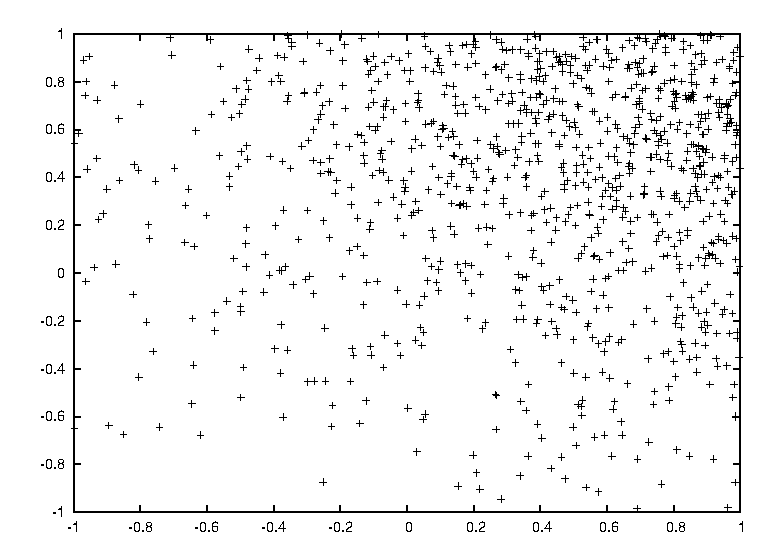
\epsfig{file=images/ballwalk_5000_cube10_cold,width=8cm}}
\subfloat[Adaptive]{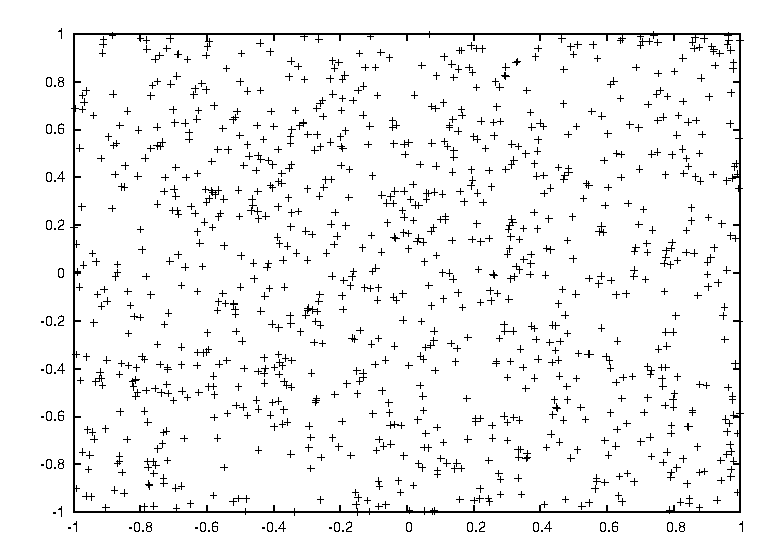
\epsfig{file=images/ballwalk_adaptive_5000_cube10_cold,width=8cm}}
\caption{5000 iteration ball walking methods on the 10 dimensional cube with a bad start}
\label{ballwalking}
\end{figure}

\begin{figure}
\centering
\subfloat[Standard]{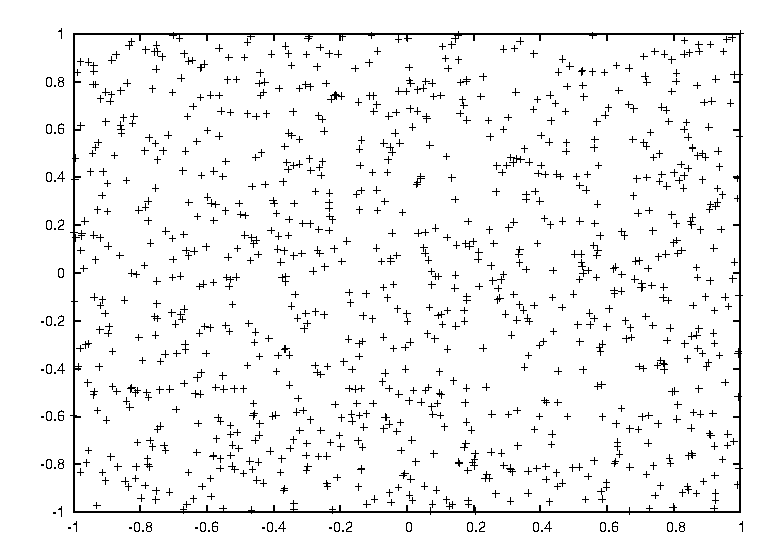
\epsfig{file=images/gaussian_5000_cube10_cold,width=8cm}}
\subfloat[Adaptive]{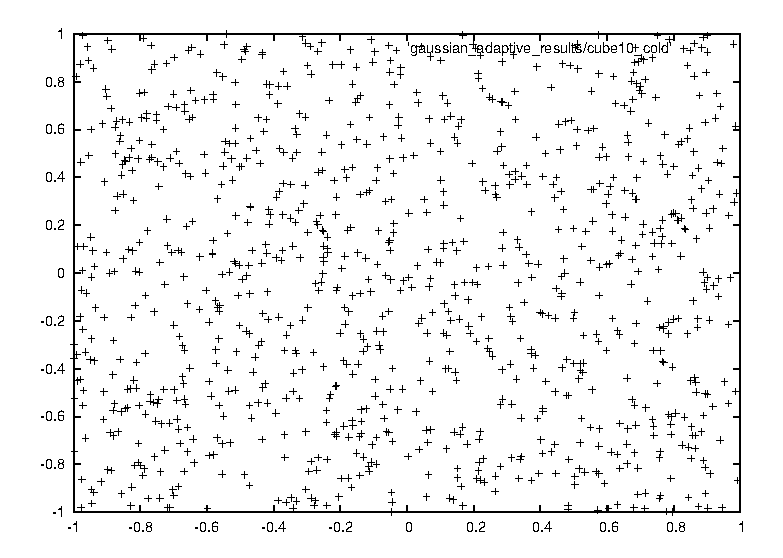
\epsfig{file=images/gaussian_adaptive_5000_cube10_cold,width=8cm}}
\caption{5000 iteration Gaussian walking methods on the 10 dimensional cube with a bad start}
\label{gaussian}
\end{figure}

\begin{figure}
\centering
\subfloat[Standard]{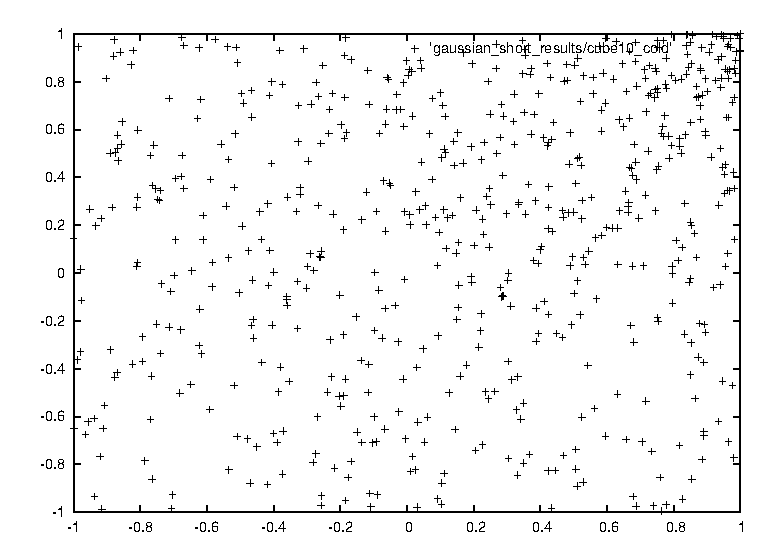
\epsfig{file=images/gaussian_2000_cube10_cold,width=8cm}}
\subfloat[Adaptive]{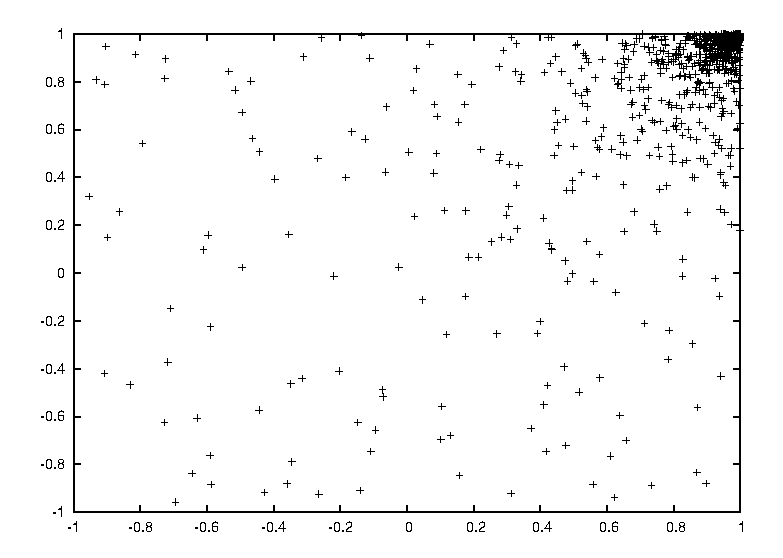
\epsfig{file=images/gaussian_adaptive_2000_cube10_cold,width=8cm}}
\caption{2000 iteration Gaussian walking methods on the 10 dimensional cube with a bad start}
\label{gaussian_short}
\end{figure}

\begin{figure}
\centering
\subfloat[Standard Ball-Walking]{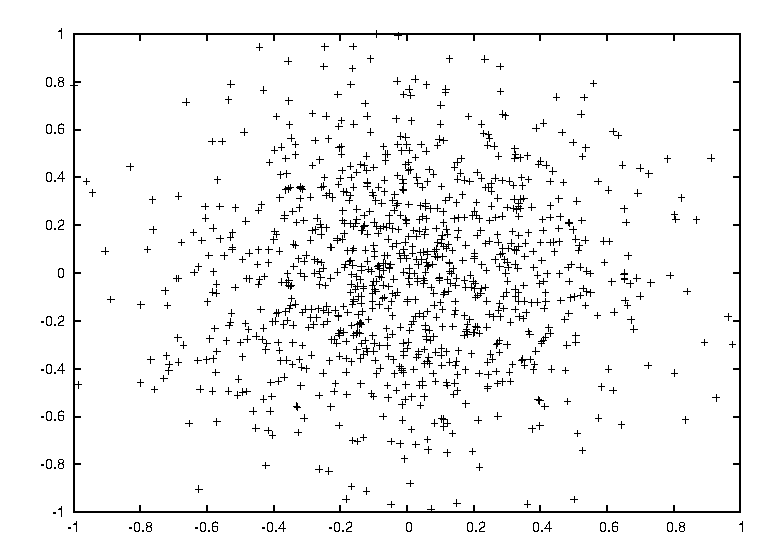
\epsfig{file=images/ballwalk_5000_cube100_warm,width=5.4cm}}
\subfloat[Adaptive Ball-Walking]{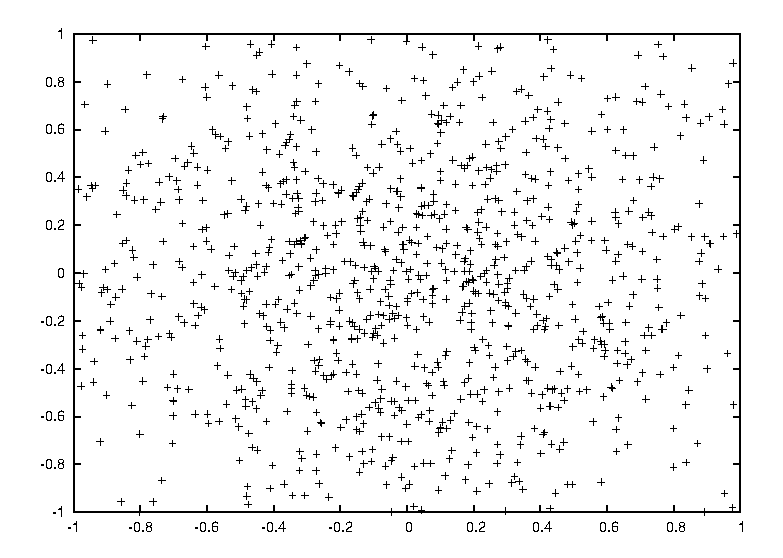
\epsfig{file=images/ballwalk_adaptive_5000_cube100_warm,width=5.4cm}}
\subfloat[Standard Gaussian-Walking]{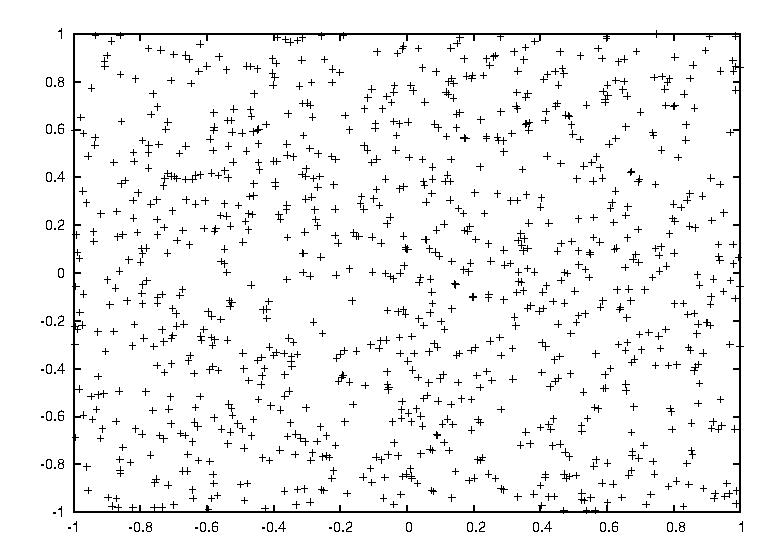
\epsfig{file=images/gaussian_5000_cube100_warm,width=5.4cm}}
\caption{5000 iteration Metropolis methods on the 100 dimensional cube with a good start}
\label{big_cube}
\end{figure}

\begin{figure}
\centering
\subfloat[10 dimensional cube, bad start]{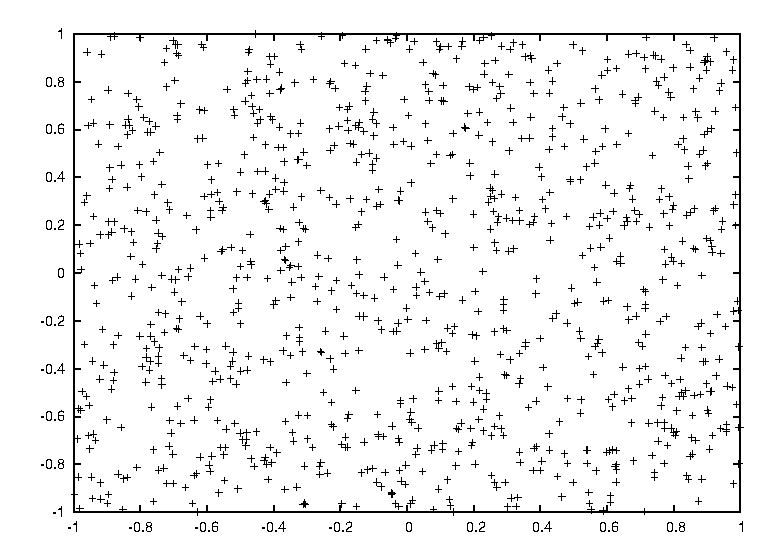
\epsfig{file=images/hitandrun_1200_cube10_cold,width=8cm}}
\subfloat[100 dimensional cube, good start]{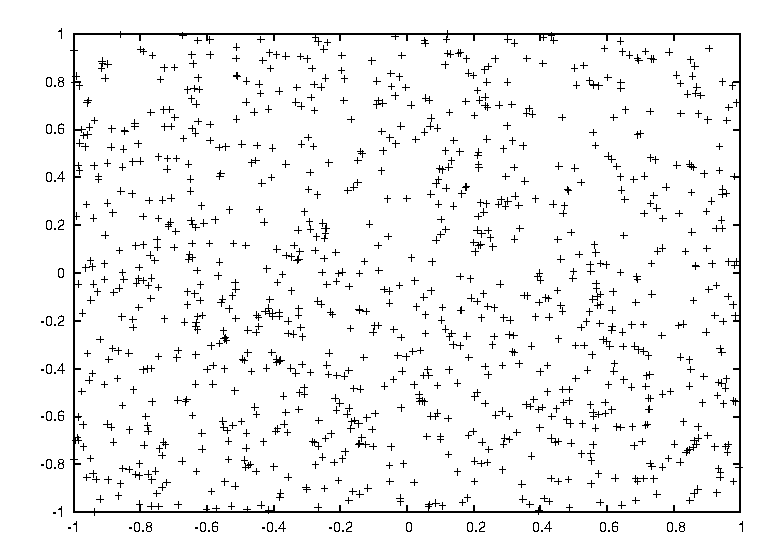
\epsfig{file=images/hitandrun_1200_cube100_warm,width=8cm}}
\caption{1200 iteration hit-and-run method on the 10 dimensional and 100 dimensional cubes}
\label{hitandrun}
\end{figure}

\begin{figure}
\centering
\subfloat[5000 Iteration Standard Ball-Walking]{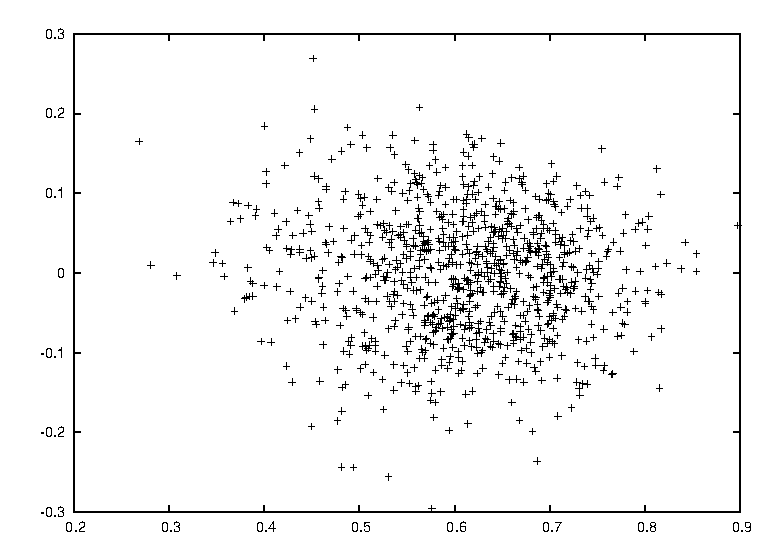
\epsfig{file=images/ballwalk_5000_sphere100_cold,width=8cm}}
\subfloat[5000 Iteration Adaptive Ball-Walking]{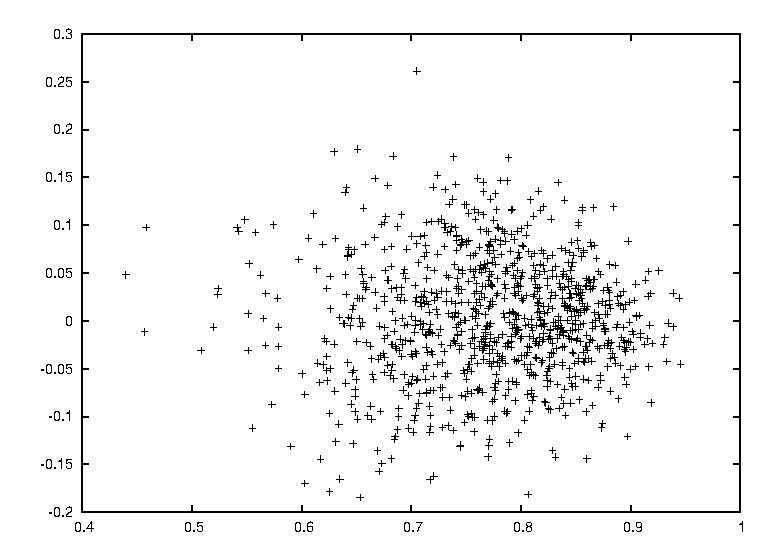
\epsfig{file=images/ballwalk_adaptive_5000_sphere100_cold,width=8cm}}

\subfloat[5000 Iteration Standard Gaussian-Walking]{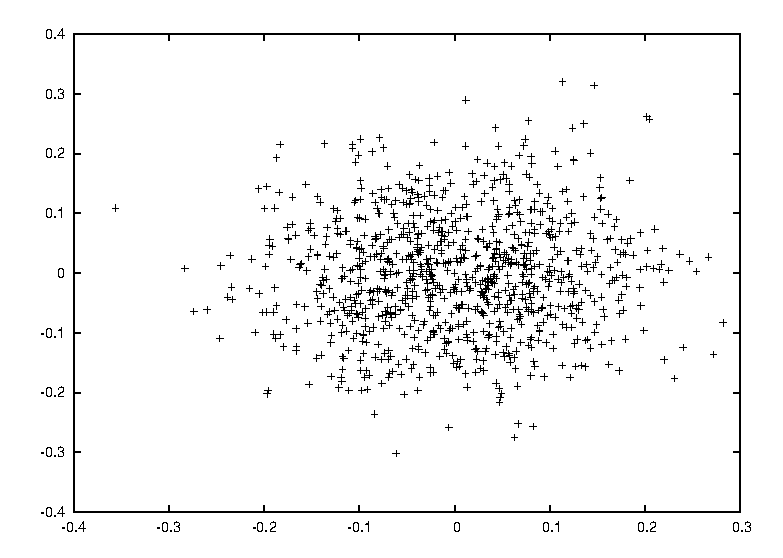
\epsfig{file=images/gaussian_adaptive_5000_sphere100_cold,width=8cm}}
\subfloat[5000 Iteration Adaptive Gaussian-Walking]{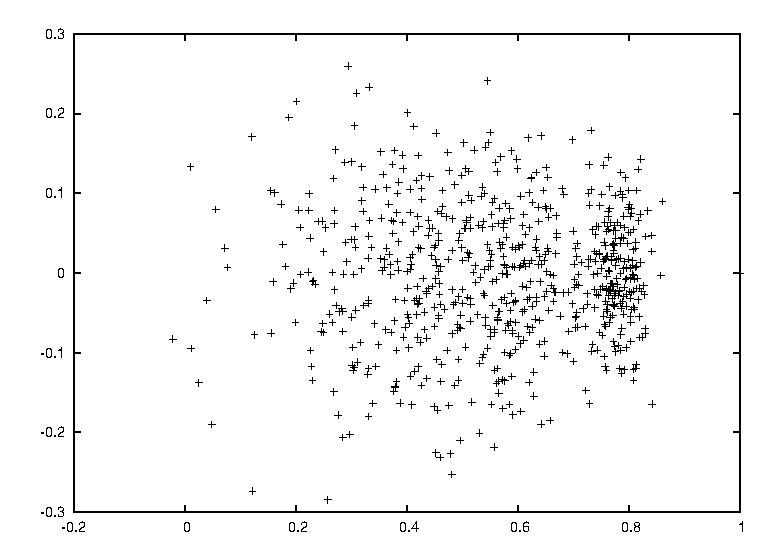
\epsfig{file=images/gaussian_5000_sphere100_cold,width=8cm}}

\subfloat[1200 Iteration Hit and Run]{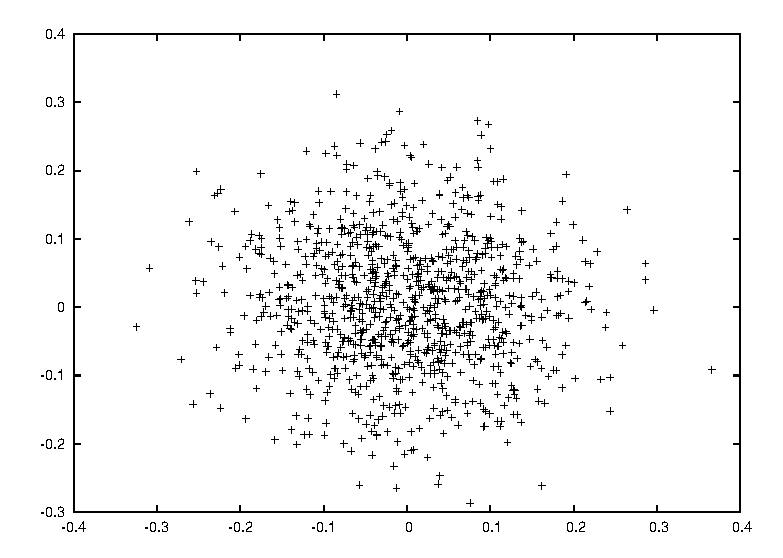
\epsfig{file=images/hitandrun_1200_sphere100_cold,width=8cm}}
\caption{Sampling methods on the 100 dimensional sphere with a bad start}
\label{sphere}
\end{figure}

\section{Conclusion}

In conclusion, we have found that the results of our tests confirm what we thought to be theoretically true: the hit-and-run method performs much better than the Metropolis methods. With a good start, hit-and-run required only something on the order of $1000$ iterations to produce a distribution that seemed reasonably uniform, which is even better than the bound given in Theorem \ref{hitandrunbound}, even with $100$ dimensions, whereas this cube is too larger for the the basic-ball walking method to have a good chance of even reaching the edges. We also saw that the basic Gaussian-walking method worked better than the ball-walking method in this case.

In general, the adaptive methods performed better than their non-adaptive counterparts. When started from the corner of a cube or a simplex, the non-adaptive methods would always stay in that corner for high-dimension test cases, even $n=10$. The adaptive methods, however, produced a distribution which looked much more uniform. However, in cases where we do not start close to a boundary, the adaptive methods do not have as much of an advantage over the non-adaptive methods.

These results indicate that, in practice, the hit-and-run method is better than the Metropolis methods, even when taking into account its slower transition step. Among the Metropolis methods, the Gaussian-walking method is a slight improvement over the ball-walking method, and the adaptive methods usually help in cases where are starting point is near a corner.

\pagebreak

\begin{thebibliography}{9}

\bibitem{Dabbene} Dabbene, F., ``A randomized cutting plane scheme for convex optimization,'' Computer-Aided Control Systems, 2008. CACSD 2008. IEEE International Conference on , vol., no., pp.120-125, 3-5 Sept. 2008.

\bibitem{Marsaglia} Marsaglia, G. and Bray, T.A. ``A Convenient Method for Generating Normal Variables." \emph{SIAM Review} Vol. 6, No. 3 (Jul., 1964), pp. 260-264.

\bibitem{Vempala} Lov\'asz, L. and Vempala, S. Hit-and-Run from a corner. \emph{SIAM Journal on Computing}, 35(4):9851005, 2006.

\bibitem{Metropolis} Metropolis, N., Rosenbluth, M.N., Teller, A.H., Teller, E. ``Equations of State Calculations by Fast Computing Machines.'' \emph{Journal of Chemical Physics} \textbf{21} (6) pp. 1087-1092, June, 1953.

\bibitem{Smith} Smith, R.L. \emph{Efficient Monte-Carlo procedures for generating points uniformly distributed over
bounded regions}, Oper. Res., 32 (1984), pp. 1296-1308.

\end{thebibliography}

\end{document}

